\documentclass[runningheads, 12pt]{llncs}

\usepackage{float}
\usepackage{hyperref}
\usepackage{graphicx}
\graphicspath{ {./images/} }
% Used for displaying a sample figure. If possible, figure files should
% be included in EPS format.
%
% If you use the hyperref package, please uncomment the following line
% to display URLs in blue roman font according to Springer's eBook style:
% \renewcommand\UrlFont{\color{blue}\rmfamily}

\begin{document}

\title{Match-three game engine}

\author{Krzysztof Rudnicki\inst{1}\orcidID{0009-0005-3306-8946}}

\authorrunning{K. Rudnicki}

\institute{Warsaw University of Technology, Warsaw plac Politechniki 1, Poland}

\maketitle           

\begin{abstract}
    Article is about creating a game engine specialized in match-three multiplatform games using OpenGL

\keywords{OpenGL  \and Game Engine \and C++}
\end{abstract}

\section{Overview}
Video games are an essential part of the digital culture, growth of mobile gaming has led to a surge in the popularity of genres like match-three games. The development of a specialized game engine for such games provides an efficient, reusable, simple and robust way to create and distribute these games on multiple platforms.

\section{Game engine architecture}
A game engine acts as the software tool simplifying the process of creating a video game. It handles vital tasks such as rendering graphics, handling user input and managing resources. When it comes to developing a game engine for match-three games, considerations need to be made to ensure the architecture is capable of handling specific requirements from this typ of game

\subsection{Game Loop} The game loop is a crucial component of the game engine, controlling the flow of the game by continuously updating game state and rendering the game to the screen \cite{ref_book1}. In the context of match-three games, the game loop should be designed to handle real-time user input and update the game board effectively.

\begin{figure}
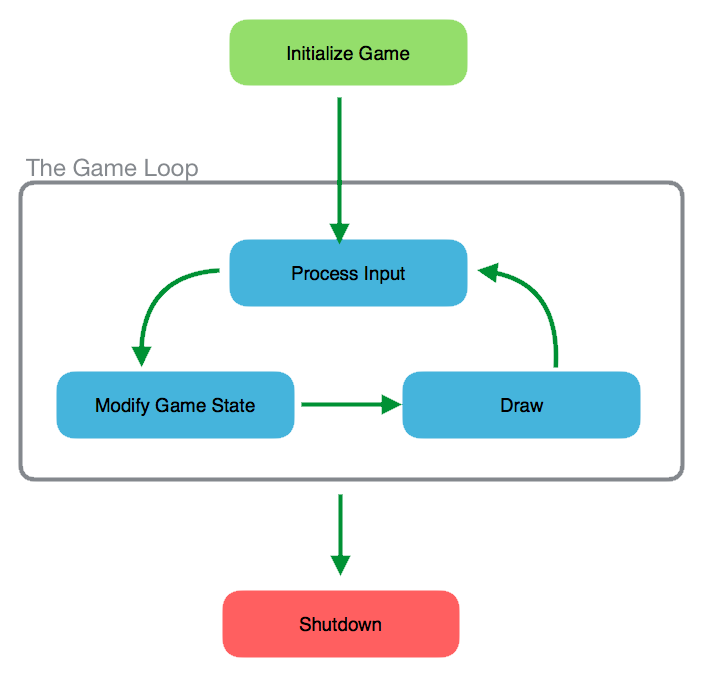
\includegraphics[width=\textwidth]{gameloop.png}
\caption{Graphical representation of game loop from \cite{ref_url3}} \label{fig1}
\end{figure}

\subsection{Entity-Component-System}
The Entity-Component-System (ECS) is a widely-used architectural pattern in game engines. ECS allows for efficient management of game objects (entities), their characteristics (components), and their behaviors (systems) \cite{ref_url1}. ECS is particularly well-suited for match-three games, where each game piece can be considered an entity, with different properties and behaviors.

\section{OpenGL and Rendering Techniques}
OpenGL is a cross-platform API that provides a wide range of functions for rendering 2D and 3D graphics \cite{ref_url2}. With OpenGL, developers can create efficient, high-performance rendering pipelines for their match-three games.

\subsection{Texture Mapping}
Texture mapping is a critical process in computer graphics that grants objects a high degree of visual complexity without an excessive increase in computational cost \cite{ref_book2}. In the context of match-three games, texture mapping can significantly enrich the visual experience by adding detailed designs and patterns to otherwise flat and monotonous game pieces, creating a more engaging and visually satisfying game environment.

\begin{figure}[H]
    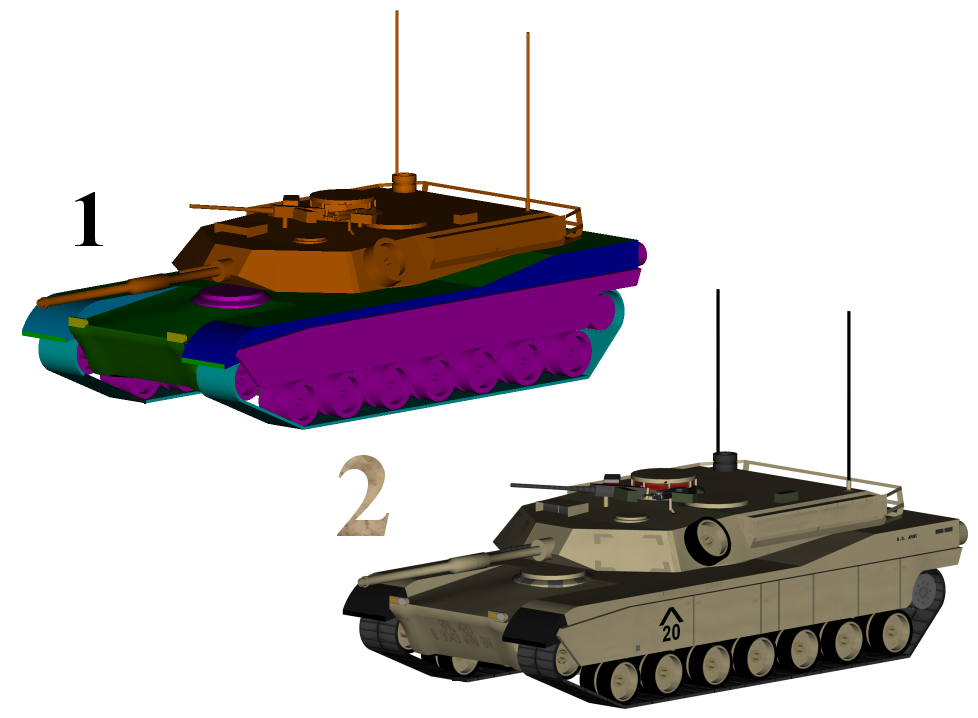
\includegraphics[width=\textwidth]{textureMapping.png}
    \caption{Tank model without and with texture from \cite{ref_url4}} \label{fig2}
    \end{figure}

\subsubsection{Basic Concepts of Texture Mapping}
Texture mapping refers to the process of wrapping or mapping a 2D image, referred to as a 'texture', onto a 3D model or surface \cite{ref_book6}. The texture contains color information, patterns, or details that should be applied to the surface of the object.

This mapping is controlled by a set of coordinates known as texture coordinates, or UV coordinates. Each point on the texture map corresponds to a point on the 3D object's surface. This correspondence is defined using these UV coordinates, which are typically normalized between 0 and 1 \cite{ref_book7}.

In match-three games, texture mapping can be utilized to apply colors, designs, or patterns to individual game pieces. For example, a simple square can be transformed into a vibrant gemstone by applying a gemstone texture.

\subsubsection{Techniques in Texture Mapping}
There are various techniques in texture mapping, such as planar mapping, cylindrical mapping, and spherical mapping \cite{ref_book8}. The selection of the technique depends on the shape and complexity of the 3D object. For match-three games, which typically use relatively simple shapes for game pieces, planar mapping is often sufficient.

\paragraph{Planar Mapping}
In planar mapping, the texture is projected onto the object like a slide projector. The X and Y coordinates of the texture correspond to two axes of the 3D object, while the Z value is ignored \cite{ref_book8}. This makes planar mapping an excellent choice for flat or box-like objects, as seen in many match-three games.

\subsubsection{Challenges in Texture Mapping}
Despite its seemingly straightforward nature, texture mapping does come with its set of challenges. Issues such as texture distortion, seams, and aliasing can significantly degrade the visual quality of the final rendering.

\paragraph{Texture Distortion}
Texture distortion occurs when the mapping from the texture to the 3D surface stretches or squashes the texture, resulting in a distorted appearance. This is often due to the difference in aspect ratio between the texture and the 3D surface \cite{ref_book2}.

\paragraph{Seams}
Seams occur at the boundaries where textures meet, particularly in the case of multiple textures on a single object. This can lead to visible discontinuities on the object's surface. In match-three games, care should be taken when mapping textures to ensure seamless transitions between game pieces.

\paragraph{Aliasing}
Aliasing, specifically texture aliasing, occurs when the texture is sampled at a lower frequency than its resolution, resulting in jagged or pixelated appearance. Techniques such as Mipmapping and Anisotropic filtering can help alleviate this issue.

\subsection{Shaders}
Shaders are programs that run on the GPU, and they control the final look of what is rendered on the screen \cite{ref_book3}. Using shaders, developers can create visually stunning effects for match-three games, such as glowing game pieces or sophisticated transition effects.

\section{Multiplatform Compatibility}
A key feature of a specialized game engine for match-three games is the ability to deploy on various platforms, including but not limited to desktop (Windows, Mac, Linux), mobile (iOS, Android), and game consoles (Xbox, PlayStation, Nintendo Switch). Achieving multiplatform compatibility calls for an understanding of various factors, including abstracting platform-specific code, implementing a robust resource management system, adapting input methods, adjusting graphical settings, and ensuring network compatibility.

\subsection{Abstracting Platform-Specific Code}
Platform-specific code deals with the low-level interactions between the game and the hardware it runs on. These interactions can include things like window creation, file system access, and input handling \cite{ref_book4}. The abstraction of this code is critical for developing a game engine with multiplatform support. Libraries such as (Graphics Library Framework) can be utilized to handle these platform-specific details.
\\ 
GLFW is specifically designed for creating windows with OpenGL contexts and managing input, making it a perfect fit for a game engine based on OpenGL.

\subsection{Implementing a Robust Resource Management System}
Managing resources like textures, sounds, and models is another key aspect of multiplatform compatibility. Each platform will have its limitations and considerations concerning memory management and file system access.

For example, a desktop PC may have a considerable amount of memory available and be able to load all resources at game startup. On the other hand, a mobile device with limited memory will require a more dynamic approach, loading and unloading resources as needed.

The game engine should have a system in place to handle these differences, abstracting the resource management away from the game developers and ensuring the most efficient use of resources on each platform.

\subsection{Adapting Input Methods}
Different platforms require different input methods. For instance, a game on a desktop might use mouse and keyboard input, while a game on a mobile device would use touch input. Console version of game will make use of console gamepad. Therefore, the game engine must provide an abstracted input system that allows game developers to handle input in a way that is independent of the actual hardware being used \cite{ref_book4}.
\\
This system can be event-driven, where the game engine generates events for different types of input (like a button press or a screen touch), and the game responds to these events. This approach allows for easy mapping of different input methods to game actions, improving the multiplatform capabilities of the game engine.

\subsection{Adjusting Graphical Settings}
Graphical performance can vary greatly between platforms. While a high-end desktop PC can handle complex graphics and high resolutions, a mobile device or older computer might struggle with the same settings. Thus, the game engine should provide ways to adjust the graphical settings based on the capabilities of the platform \cite{ref_book5}.
\\ 
This could involve creating different levels of detail for models and textures, allowing for dynamic resolution scaling, or providing options to enable or disable various graphical effects.


\section{Summary}
The creation of a specialized game engine for match-three games requires careful consideration of various factors, such as game engine architecture, rendering techniques, multiplayer functionalities, and multiplatform compatibility. With appropriate design and implementation, such an engine can significantly streamline the development of match-three games across platforms.

\section{References / Sources}
\begin{thebibliography}{8}

    \bibitem{ref_book1}
Author, John P. Doran. Author, Matt Casanova: Game Development Patterns and Best Practices. Packt Publishing, (2017)

\bibitem{ref_url1}
Data Oriented Design, Noel Llopis, \url{https://gamesfromwithin.com/data-oriented-design}. Last accessed 16
Jun 2023

\bibitem{ref_url2}
Khronos Group. OpenGL main page
\url{https://www.opengl.org/}, Last acceessed 16 Jun 2023

\bibitem{ref_url3}
BYU-Idaho. CS 165 introduction
\url{https://content.byui.edu/file/2315e65e-a34a-48d3-814d-4175a2b74ed5/1/intro/165-gameloop.html}, Last acceessed 16 Jun 2023

\bibitem{ref_url4}
Wikipedia, Texture Mapping
\url{https://en.wikipedia.org/wiki/Texture_mapping}, Last accessed 16 Jun 2023

\bibitem{ref_book2}
Author, Eric Haines. Author, Tomas Möller, Naty Hoffman: Real-Time Rendering 1st edition. CRC Press, (1999)

\bibitem{ref_book3}
Author,  Randi J. Rost: OpenGL Shading Language book 3rd edition. Pearson Education, (2009)

\bibitem{ref_book4}
Author, Jason Gregory: Game Engine Architecture 3rd edition. CRC Press. (2018) 

\bibitem{ref_book5}
Author, Steven Goodwin: Cross-platform Game Programming. Charles River Media. (2005) 

\bibitem{ref_book6}
Author, Edward Angel. Author Dave Shreiner: Interactive Computer Graphics. A Top-Down Approach with WebGL. Pearson (2014)

\bibitem{ref_book7}
Author, Alan Watt: 3D Computer Graphics 3rd edition. Addison-Wesley (1999)

\bibitem{ref_book8}
Author, Donald D. Hearn. Author, Pauline Baker. Author, Warren Carithers: Computer Graphics with Open GL. Pearson (2013)



\end{thebibliography}
\end{document}
